%; whizzy paragraph -pdf xpdf -latex ./whizzypdfptex.sh
%; whizzy-paragraph "^\\\\begin{frame}"
% latex beamer presentation.
% platex, latex-beamer $B$G%3%s%Q%$%k$9$k$3$H$rA[Dj!#(B 

%     Tokyo Debian Meeting resources
%     Copyright (C) 2009 Junichi Uekawa
%     Copyright (C) 2009 Nobuhiro Iwamatsu

%     This program is free software; you can redistribute it and/or modify
%     it under the terms of the GNU General Public License as published by
%     the Free Software Foundation; either version 2 of the License, or
%     (at your option) any later version.

%     This program is distributed in the hope that it will be useful,
%     but WITHOUT ANY WARRANTY; without even the implied warranty of
%     MERCHANTABILITY or FITNESS FOR A PARTICULAR PURPOSE.  See the
%     GNU General Public License for more details.

%     You should have received a copy of the GNU General Public License
%     along with this program; if not, write to the Free Software
%     Foundation, Inc., 51 Franklin St, Fifth Floor, Boston, MA  02110-1301 USA

\documentclass[cjk,dvipdfmx,12pt]{beamer}
\usetheme{Tokyo}
\usepackage{monthlypresentation}

%  preview (shell-command (concat "evince " (replace-regexp-in-string "tex$" "pdf"(buffer-file-name)) "&"))
%  presentation (shell-command (concat "xpdf -fullscreen " (replace-regexp-in-string "tex$" "pdf"(buffer-file-name)) "&"))
%  presentation (shell-command (concat "evince " (replace-regexp-in-string "tex$" "pdf"(buffer-file-name)) "&"))

%http://www.naney.org/diki/dk/hyperref.html
%$BF|K\8l(BEUC$B7O4D6-$N;~(B
\AtBeginDvi{\special{pdf:tounicode EUC-UCS2}}
%$B%7%U%H(BJIS$B7O4D6-$N;~(B
%\AtBeginDvi{\special{pdf:tounicode 90ms-RKSJ-UCS2}}

\title{Debian $B$G$N?t3X$3$H$O$8$a!#(B}
\subtitle{gnuplot, Octave, R $BF~Lg(B}
\author{$B$^$($@$3$&$X$$(B mkouhei@debian.or.jp \\IRC nick: mkouhei}
\date{2009$BG/(B11$B7n(B14$BF|(B}
\logo{
\includegraphics[width=8cm]{image200607/openlogo-light.eps}}

%begin of commandline0
\newenvironment{commandline0}%
{\VerbatimEnvironment
  \begin{Sbox}\begin{minipage}{0.9\hsize}\begin{fontsize}{5}{5} \begin{BVerbatim}}%
{\end{BVerbatim}\end{fontsize}\end{minipage}\end{Sbox}
  \setlength{\fboxsep}{10pt}

\vspace{10pt}% skip before
\fcolorbox{dancerdarkblue}{dancerlightblue}{\TheSbox}

\vspace{6pt}% skip after
}
%end of commandline0

\begin{document}

\frame{\titlepage{}}

\begin{frame}{$B%9%W%l%C%I%7!<%H$C$FMn$A$^$;$s!)(B}
\begin{itemize}
 \item $B%G!<%?NLA}$($F$/$k$H%l%9%]%s%9:G0-!#(B
 \item $B=[4D;2>H$9$k$H(BOOo$B$J$s$FMn$A$k!#(B
 \item OS$B$^$G8G$^$k$J$s$F:G0-!#(B
\end{itemize}

$B$=$NB>$NITK~!#(B
\begin{itemize}
 \item $BAH$_9~$_4X?t$N@:EY$,$=$b$=$b2x$7$$!#(B
 \item $B%F%-%9%H%G!<%?$8$c$J$$$+$i!"(Bdiff $B$G$-$J$$$7!#(B\\
       \texttt{git diff --binary}$B$G$-$k$1$I!"FI$a$s!*(B
\end{itemize}
\end{frame}

\begin{frame}{$B:2$N6+$S$,J9$3$($=$&$G$9!#(B}
 \begin{minipage}[t]{0.45\hsize}
  \huge{$B$b$&$3$s$J@83h7y$@!*(B}
 \end{minipage}
 \begin{minipage}[t]{0.45\hsize}
  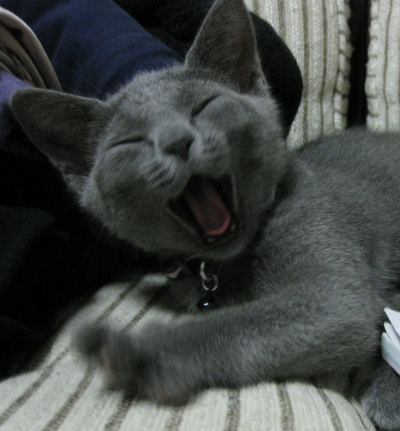
\includegraphics[width=1\hsize]{image200911/komame.png}
 \end{minipage}
\end{frame}

\begin{frame}{$B:#F|$N8%N)!#(B}
\begin{itemize}
\item gnuplot
\item GNU Octave
\item GNU R
\end{itemize}

$B0J>e!";0K\$r$*Aw$j$7$^$9!#(B
\end{frame}

\begin{frame}{$BFCD'!#(B}
\begin{itemize}
 \item gnuplot
      \begin{itemize}
       \item $B%0%i%UIA2h$,F@0U$J%3!#(B
       \item $B30It%W%m%0%i%`$+$i8F$S=P$;$^$9!#(B
       \item LaTeX$B$H$bO"7H$G$-$A$c$$$^$9!#(B
      \end{itemize}
 \item GNU Octave
       \begin{itemize}
	\item $B?tCM7W;;$,F@0U$J%3!#(B
	\item $B%0%i%UIA2h$O(B gnuplot $B;H$$$^$9!#(B
	\item MATLAB $B$N8_49$rL\;X$7$F$^$9!#(B\footnote{$BJL$N8+J}$G$O(BMATLAB
	      $B$N%/%m!<%s(B(clone)$B$J$s$@$H$+!#(B}
       \end{itemize}
 \item GNU R
       \begin{itemize}
	\item $BE}7W=hM}$,F@0U$J%3!#(B
	\item $B3HD%5!G=$,K-IY$G$9!#(B
	\item $B%0%i%UIA2h5!G=$b$"$j$^$9!#(B
       \end{itemize}
\end{itemize}
\end{frame}

\begin{frame}[containsverbatim]{$B%$%s%9%H!<%kJ}K!!#(B}
gnuplot

\begin{commandline}
$ sudo apt-get install gnuplot
\end{commandline}

GNU Octave

\begin{commandline}
$ sudo apt-get install octave3.2
\end{commandline}

GNU R

\begin{commandline}
$ sudo apt-get install r-base
\end{commandline}

\end{frame}

\begin{frame}[containsverbatim]{$B:#7n$N6q:`!#(B}
$B2f$,2H$N8wG.Hq(B
\begin{commandline}
"date","days","kWh","kWh/d","yen/d","yen","days","m^3","m^3/d","yen/d","yen","days","m^3","m^3/d","yen/d","yen","yen/d","yen"
2001/04,11,34,3.09,83.5,918,36,4.9,0.14,108.3,3900,58,9,0.16,22.8,1320,,
2001/05,33,95,2.88,73.8,2434,29,3.5,0.12,114.1,3310,,,,,,,
2001/06,30,129,4.3,102.7,3082,32,3,0.09,96.9,3100,61,3,0.05,15.7,960,,
2001/07,28,155,5.54,131.3,3676,28,1.7,0.06,91.1,2550,,,,,,,
(snip)
\end{commandline}

 image200911/konetsu.csv $B$K$"$k$N$G!"<j85$KJY6/2q$N%j%]%8%H%j$,$"$k?M$O;n(B
 $B$7$F$_$k$HNI$$$h!#(B
\end{frame}

\begin{frame}{$B:#7n$N6q:`!#(B}
$B2f$,2H$N8wG.Hq(B
\begin{itemize}
 \item 2001$BG/(B4$B7n$+$i(B2009$BG/(B9$B7n$^$G$N%G!<%?!#(B
 \item 2$B2sBg$-$/JQ$o$k!#Bg;(GD$KGD0.$7$F$$$k$N$O!"0J2<!#(B
 \item 2006$BG/(B9$B7n$K;T@n$+$iB?K`$K0z1[$7!#(B
       \begin{itemize}
	\item $BEE5$7@Ls$,(B30A$B$+$i(B40A$B$K!#(B
	\item $B%,%9$,%W%m%Q%s$+$iET;T%,%9$K!#(B
	\item $B?eF;Be$,>e$,$k!u2<?eF;Be$,DI2C$K!#(B
       \end{itemize}
 \item 2008$BG/(B10$B7n$K7k:'!#(B
       \begin{itemize}
	\item $B%,%9!"?eF;;HMQNL$,G\A}!#(B
	\item $BEE5$;HMQNL$O$"$^$jJQ$o$i$:!#(B
       \end{itemize}
\end{itemize}
\end{frame}


\begin{frame}[containsverbatim]{gnuplot$B$G=hM}$7$?>l9g!#(B}
$B4pK\$O!"%G!<%?$N%W%m%C%H!#(B\\
set$B$G9T$C$F$$$k$N$O%0%i%U$N8+1I$($,<g!#(B

 \begin{minipage}{0.45\hsize}
 \begin{commandline0}
reset
set terminal epslatex input color
set output "gnuplot.tex"
set datafile separator ","
set xdata time
set timefmt "%Y/%m"
set format x "%Y/%m"
set xtics rotate by -90
set mxtics 12
set xrange ["2001/04":"2009/08"]
set yrange [0:400]
set xlabel "$BG/7n(B"
set ylabel "$BEE5$;HMQNL(B [kWh]"
set y2range [0:50]
set y2label "$B%,%9!&?eF;;HMQNL(B [$BN)J}%a!<%H%k(B]"
set ytics nomirror
set y2tics
plot "kohnetsuhi.csv" using 1:3 axes x1y1 \
  title "$BEE5$(B" with line,\
  "" using 1:8 axes x1y2 title "$B%,%9(B" with line,\
  "" using 1:13 axes x1y2 title "$B?eF;(B" with line
 \end{commandline0}
 \end{minipage}
 \begin{minipage}{0.45\hsize}
  \scalebox{0.5}[0.5]{% GNUPLOT: LaTeX picture with Postscript
\begingroup
  \makeatletter
  \providecommand\color[2][]{%
    \GenericError{(gnuplot) \space\space\space\@spaces}{%
      Package color not loaded in conjunction with
      terminal option `colourtext'%
    }{See the gnuplot documentation for explanation.%
    }{Either use 'blacktext' in gnuplot or load the package
      color.sty in LaTeX.}%
    \renewcommand\color[2][]{}%
  }%
  \providecommand\includegraphics[2][]{%
    \GenericError{(gnuplot) \space\space\space\@spaces}{%
      Package graphicx or graphics not loaded%
    }{See the gnuplot documentation for explanation.%
    }{The gnuplot epslatex terminal needs graphicx.sty or graphics.sty.}%
    \renewcommand\includegraphics[2][]{}%
  }%
  \providecommand\rotatebox[2]{#2}%
  \@ifundefined{ifGPcolor}{%
    \newif\ifGPcolor
    \GPcolortrue
  }{}%
  \@ifundefined{ifGPblacktext}{%
    \newif\ifGPblacktext
    \GPblacktexttrue
  }{}%
  % define a \g@addto@macro without @ in the name:
  \let\gplgaddtomacro\g@addto@macro
  % define empty templates for all commands taking text:
  \gdef\gplbacktext{}%
  \gdef\gplfronttext{}%
  \makeatother
  \ifGPblacktext
    % no textcolor at all
    \def\colorrgb#1{}%
    \def\colorgray#1{}%
  \else
    % gray or color?
    \ifGPcolor
      \def\colorrgb#1{\color[rgb]{#1}}%
      \def\colorgray#1{\color[gray]{#1}}%
      \expandafter\def\csname LTw\endcsname{\color{white}}%
      \expandafter\def\csname LTb\endcsname{\color{black}}%
      \expandafter\def\csname LTa\endcsname{\color{black}}%
      \expandafter\def\csname LT0\endcsname{\color[rgb]{1,0,0}}%
      \expandafter\def\csname LT1\endcsname{\color[rgb]{0,1,0}}%
      \expandafter\def\csname LT2\endcsname{\color[rgb]{0,0,1}}%
      \expandafter\def\csname LT3\endcsname{\color[rgb]{1,0,1}}%
      \expandafter\def\csname LT4\endcsname{\color[rgb]{0,1,1}}%
      \expandafter\def\csname LT5\endcsname{\color[rgb]{1,1,0}}%
      \expandafter\def\csname LT6\endcsname{\color[rgb]{0,0,0}}%
      \expandafter\def\csname LT7\endcsname{\color[rgb]{1,0.3,0}}%
      \expandafter\def\csname LT8\endcsname{\color[rgb]{0.5,0.5,0.5}}%
    \else
      % gray
      \def\colorrgb#1{\color{black}}%
      \def\colorgray#1{\color[gray]{#1}}%
      \expandafter\def\csname LTw\endcsname{\color{white}}%
      \expandafter\def\csname LTb\endcsname{\color{black}}%
      \expandafter\def\csname LTa\endcsname{\color{black}}%
      \expandafter\def\csname LT0\endcsname{\color{black}}%
      \expandafter\def\csname LT1\endcsname{\color{black}}%
      \expandafter\def\csname LT2\endcsname{\color{black}}%
      \expandafter\def\csname LT3\endcsname{\color{black}}%
      \expandafter\def\csname LT4\endcsname{\color{black}}%
      \expandafter\def\csname LT5\endcsname{\color{black}}%
      \expandafter\def\csname LT6\endcsname{\color{black}}%
      \expandafter\def\csname LT7\endcsname{\color{black}}%
      \expandafter\def\csname LT8\endcsname{\color{black}}%
    \fi
  \fi
  \setlength{\unitlength}{0.0500bp}%
  \begin{picture}(7200.00,5040.00)%
    \gplgaddtomacro\gplbacktext{%
      \csname LTb\endcsname%
      \put(1210,1408){\makebox(0,0)[r]{\strut{} 0}}%
      \put(1210,1829){\makebox(0,0)[r]{\strut{} 50}}%
      \put(1210,2250){\makebox(0,0)[r]{\strut{} 100}}%
      \put(1210,2671){\makebox(0,0)[r]{\strut{} 150}}%
      \put(1210,3092){\makebox(0,0)[r]{\strut{} 200}}%
      \put(1210,3513){\makebox(0,0)[r]{\strut{} 250}}%
      \put(1210,3934){\makebox(0,0)[r]{\strut{} 300}}%
      \put(1210,4355){\makebox(0,0)[r]{\strut{} 350}}%
      \put(1210,4776){\makebox(0,0)[r]{\strut{} 400}}%
      \put(1763,1276){\rotatebox{-90}{\makebox(0,0)[l]{\strut{}2002/01}}}%
      \put(2320,1276){\rotatebox{-90}{\makebox(0,0)[l]{\strut{}2003/01}}}%
      \put(2877,1276){\rotatebox{-90}{\makebox(0,0)[l]{\strut{}2004/01}}}%
      \put(3436,1276){\rotatebox{-90}{\makebox(0,0)[l]{\strut{}2005/01}}}%
      \put(3994,1276){\rotatebox{-90}{\makebox(0,0)[l]{\strut{}2006/01}}}%
      \put(4551,1276){\rotatebox{-90}{\makebox(0,0)[l]{\strut{}2007/01}}}%
      \put(5107,1276){\rotatebox{-90}{\makebox(0,0)[l]{\strut{}2008/01}}}%
      \put(5667,1276){\rotatebox{-90}{\makebox(0,0)[l]{\strut{}2009/01}}}%
      \put(6122,1408){\makebox(0,0)[l]{\strut{} 0}}%
      \put(6122,2082){\makebox(0,0)[l]{\strut{} 10}}%
      \put(6122,2755){\makebox(0,0)[l]{\strut{} 20}}%
      \put(6122,3429){\makebox(0,0)[l]{\strut{} 30}}%
      \put(6122,4102){\makebox(0,0)[l]{\strut{} 40}}%
      \put(6122,4776){\makebox(0,0)[l]{\strut{} 50}}%
      \put(440,3092){\rotatebox{90}{\makebox(0,0){\strut{}$BEE5$;HMQNL(B [kWh]}}}%
      \put(6759,3092){\rotatebox{90}{\makebox(0,0){\strut{}$B%,%9!&?eF;;HMQNL(B [$BN)J}%a!<%H%k(B]}}}%
      \put(3666,154){\makebox(0,0){\strut{}$BG/7n(B}}%
    }%
    \gplgaddtomacro\gplfronttext{%
      \csname LTb\endcsname%
      \put(5003,4603){\makebox(0,0)[r]{\strut{}$BEE5$(B}}%
      \csname LTb\endcsname%
      \put(5003,4383){\makebox(0,0)[r]{\strut{}$B%,%9(B}}%
      \csname LTb\endcsname%
      \put(5003,4163){\makebox(0,0)[r]{\strut{}$B?eF;(B}}%
    }%
    \gplbacktext
    \put(0,0){\includegraphics{image200911/gnuplot.eps}}%
    \gplfronttext
  \end{picture}%
\endgroup
}
 \end{minipage}
\end{frame}

\begin{frame}[containsverbatim]{gnuplot$B$G=hM}$7$?>l9g!#(B}
$B4pK\$O!"%G!<%?$N%W%m%C%H!#(B\\
set$B$G9T$C$F$$$k$N$O%0%i%U$N8+1I$($,<g!#(B

 \begin{commandline0}
reset                                        # $B@_Dj$N=i4|2=(B
set terminal epslatex input color            # EPS LaTeX $B$G%+%i!<=PNO(B
set output "gnuplot.tex"                     # $B%U%!%$%kL>(B gnuplot.tex $B$GJ]B8(B
set datafile separator ","                   # $BFI$_9~$`%G!<%?%U%!%$%k$O%+%s%^6h@Z$j(B
set xdata time                               # x$B<4$N%Q%i%a!<%?$O;~4V%G!<%?(B
set timefmt "%Y/%m"                          # $BFI$_9~$`;~4V%G!<%?$N=q<0(B
set format x "%Y/%m"                         # $B=PNO$9$k(Bx$B<4$N=q<0$r;XDj(B
set xtics rotate by -90                      # x$B<4$N%a%b%j%i%Y%k$r(B-90$BEY2sE>(B
set mxtics 12                                # x$B<4$NJd=u%a%b%j$N4V3V(B
set xrange ["2001/04":"2009/08"]             # x$B<4$N%G!<%?HO0O(B
set yrange [0:400]                           # y$B<4$N%G!<%?HO0O(B
set xlabel "$BG/7n(B"                            # x $B<4$N%i%Y%k(B
set ylabel "$BEE5$;HMQNL(B [kWh]"                 # y$B<4$NL>A0(B
set y2range [0:50]                           # $BBh(B2y$B<4$N%G!<%?HO0O(B
set y2label "$B%,%9!&?eF;;HMQNL(B [$BN)J}%a!<%H%k(B]"  # $BBh(B2y$B<4$N%i%Y%k(B
set ytics nomirror                           # $BBh(B2y$B<4$O1&B&$N$_$KI=<((B
set y2tics                                   # $BBh(B2y$B<4$rI=<((B
plot "kohnetsuhi.csv" using 1:3 axes x1y1 \  # $BBh(B1,3$BNs$N%G!<%?$G(Bx$B<4!"(By$B<4$GI=<((B
  title "$BEE5$(B" with line,\                    # $BK^Nc$N%?%$%H%k$H@~%W%m%C%H(B
  "" using 1:8 axes x1y2 title "$B%,%9(B" with line,\ 
  "" using 1:13 axes x1y2 title "$B?eF;(B" with line
 \end{commandline0}
\end{frame}

\begin{frame}[containsverbatim]{gnuplot$B$G$N=hM}!#(B}
gnuplot $B$r5/F0$7$F%P%C%A$r%m!<%I!#(B

\begin{commandline}
$ gnuplot
> load ``gnuplot.gp''
> exit
$ ls
gnuplot.eps gnuplot.tex
\end{commandline}

$B$3$l$r(B LaTeX$B$G<h$j9~$`$H!"@h$[$I$N$h$&$J?^$K!#(B
\begin{itemize}
 \item $B%G%U%)%k%H$G$O!"JL%&%#%s%I%&$GI=<($5$l$k!#(B
 \item 3$B<!85%0%i%U$J$i%0%k%0%k2sE>$b$G$-$k!#(B
 \item $BB>$N2hA|%U%)!<%^%C%H$K$b=PNO$G$-$k!#(B
\end{itemize}
\end{frame}

\begin{frame}[containsverbatim]{GNU R$B$G$N=hM}!#(B}
$B%G!<%?$N<h$j9~$_!#(B
\begin{commandline}
$ R
> konetsu <- read.csv("konetsu.csv")
\end{commandline}

$B%G!<%?$N%W%m%C%H!#(B
\begin{commandline}
> plot(konetsu$kWh, type="l", ylim=c(0,400), ann=F)
> par(new=T)
> plot(konetsu$m.3, type="l", ylim=c(0,400), ann=F, col="red")
> par(new=T)
> plot(konetsu$m.3.1, ylim=c(0,400), ann=F, col="blue")
\end{commandline}
\end{frame}

\begin{frame}{GNU R$B$G$N=hM}!#(B}
 \begin{minipage}{0.45\hsize}
\begin{figure}[H]
 \includegraphics[width=0.9\hsize]{image200911/gnur.eps}
\end{figure}
\end{minipage}
 \begin{minipage}{0.45\hsize}
gnuplot $B$N$H$-$KHf$Y!"(B
\begin{itemize}
 \item $BBh(B2y$B<4$rI=<($7$F$$$J$$!#(B
 \item $B%i%Y%kI=<($7$F$$$J$$!#(B
\item $B?eF;;HMQNL$,@~$8$c$J$$!#(B
\end{itemize}
$B$H$$$C$?$N$O!"(BGNU R$B$N$;$$$G$O$"$j$^$;$s!#(B\\
$B;d$N%+%k%^$,B-$j$J$$$@$1$G$9!#(B
\end{minipage}

\end{frame}

\begin{frame}[containsverbatim]{GNU R$B$G$N=hM}!#(B}
$BEE5$$H%,%9$N;HMQNL$NAj4X4X78$r8+$F$_$k!#(B
\begin{commandline}

> cor.test(konetsu$kWh, konetsu$m.3)

	Pearson's product-moment correlation

data:  konetsu$kWh and konetsu$m.3 
t = 1.3154, df = 100, p-value = 0.1914
alternative hypothesis: true correlation is not equal to 0 
95 percent confidence interval:
 -0.06572595  0.31685457 
sample estimates:
      cor 
0.1304159 
\end{commandline}
 $B$^$"!"J,$+$C$F$$$?$3$H$G$9$,$+$J$jDc$$$G$9!#J?6Q5$29$H$J$i!"$$$:$l$+$OAj(B
 $B4X4X78$,$"$k$+$b$7$l$^$;$s!#(B
\end{frame}

\begin{frame}{GNU Octave $B$G$N=hM}!#(B}

{\huge $BNO5Z$P$:!#(B}

\end{frame}

\emtext{Debian $B%Q%C%1!<%82=$K4X$7$F!#(B}
\begin{frame}{$B3HD%%Q%C%1!<%8$"$j$^$9!#(B}
 \begin{itemize}
  \item GNU Octave $B$O!"(BOctave-Forge$B!#(B
  \item GNU R$B$O!"(BCRAN(the Conprehensive R Archive Network)
  \item Perl $B$N(BCPAN$B$N$h$&$J$b$s!#(B
 \end{itemize}
\end{frame}

\begin{frame}[containsverbatim]{$B3HD%%Q%C%1!<%8$r(B deb $B%Q%C%1!<%8$K$9$k!#(B}
$B4{$K7k9=(Bdeb$B%Q%C%1!<%8$K$J$C$F$$$k$1$IA4$F$8$c$J$$!#(B
\begin{commandline}
$ apt-cache search "GNU R" | wc -l
213
$ apt-cache search octave | wc -l
133
\end{commandline}

\end{frame}

\begin{frame}{$B3HD%%Q%C%1!<%8$r(B deb $B%Q%C%1!<%8$K$9$k!#(B}
 deb $B%Q%C%1!<%8$K$9$k$?$a$N%Q%C%1!<%8$,MQ0U$5$l$F$$$k!#(B
 \begin{itemize}
  \item Octave $B$O!"(Boctave-pkg-dev$B!#(B
	\begin{itemize}
	 \item debian/control $B$N(B Build-Depends $B$K(B octave-pkg-dev, \\
	       Depends $B$K(B \$\{octave\:Depends\}$B$rDI5-!#(B
	 \item debian/rues $B$K(B ``include
	       /usr/share/cdbs/1/class/octave-pkg.mk''$B$rDI5-!#(B
	 \item Octave-Forge$BM3Mh$G$J$$>l9g$O!"(Brules$B$K(B ``SOURCEFORGE=NO''
	       $B$rDI5-!#(B
	\end{itemize}
  \item R $B$O!"(B r-base-dev$B!#(B
	\begin{itemize}
	 \item Debian $B%Q%C%1!<%8%]%j%7!<$r9MN8$7$F!"%P%$%J%j7A<0$N<B9T%U%!(B
	       $B%$%k$O!"(B/usr/lib/R/bin/R.binary$B$KJ,N%$9$kI,MW$,$"$k!#(B
	 \item $B$H$"$C$?$N$@$1$I!"$h$/J,$+$i$:!#(BJava$B$N$h$&$K%P%$%J%j%3!<(B
	       $B%I$GG[I[$5$l$F$$$k!"$H$$$&$3$H$@$m$&$+!)(B
	 \item $B65$($F!"%(%m$$%R%H!#(B
	\end{itemize}
\end{itemize}
\end{frame}

\begin{frame}{$B$^$H$a(B}
\begin{itemize}
 \item gnuplot, GNU R, GNU Octave $B$NF3F~J}K!!#(B
 \item gnuplot, GNU R $B$N4JC1$J;H$$J}!#(B
 \item $B3HD%%Q%C%1!<%8$N(B Debian $B%Q%C%1!<%82=$N:]$N9MN8!#(B
 \item $BE}7W=hM}$K$D$$$F$O!"7n$NJ?6Q5$29$H$NAj4X4X78$r=P$9$D$b$j$@$C$?!#(B
 \item $B$,!"5$>]D#$N%G!<%?$+$i0z$CD%$C$F$/$k$N$O7k9=LLE]$J$N$G!":#8e$d$C$F$_$k!#(B
\end{itemize}

\end{frame}


\end{document}

;;; Local Variables: ***
;;; outline-regexp: "\\([ 	]*\\\\\\(documentstyle\\|documentclass\\|emtext\\|section\\|begin{frame}\\)\\*?[ 	]*[[{]\\|[]+\\)" ***
;;; End: ***
